\chapter{Tic-Tac-Toe}

\section{Rules}
\emph{Tic-tac-toe} is played on a \(3\times 3\) grid of empty squares. Two
players take turns; one uses the mark \textbf{X} and the other \textbf{O}.
Traditionally X moves first.

\begin{itemize}
  \item On your turn you place your mark in any \emph{empty} square.
  \item The game ends as soon as one player has three of their marks in a
  straight line---horizontally, vertically, or diagonally---or when all nine
  squares are filled.
  \item Three in a row wins; if the board is full with no winner, the game is a
  \emph{draw}.
\end{itemize}

\section{Positions and the game tree}
Every way the board can look (together with whose turn it is) is a
\emph{position}. A \emph{move} takes one legal position to another by adding a
single mark in an empty cell.

Imagine drawing a diagram whose \emph{nodes} are positions and whose
\emph{edges} are moves. Start from the empty board at the \emph{root}. From each
node, draw one branch downward for each legal move; that gives a (very large)
\emph{game tree}. Leaves are terminal positions: someone has won or every cell
is full.

The tree is finite: there are only finitely many boards, and each game lasts at
most nine moves, so every path from the root eventually stops.

\section{Finding the best move with a tree}
To decide the \emph{best} move from a given position, assume both players play
as well as possible from then on. We attach a \emph{score} to each terminal
position from the point of view of the player who is about to move at the root
of the subtree we are evaluating (fix that player once and for all---say
\textbf{X}):

\begin{itemize}
  \item If X wins the terminal position, score \(+1\).
  \item If O wins, score \(-1\).
  \item If the game is a draw, score \(0\).
\end{itemize}

Work \emph{backward} from the leaves:

\begin{itemize}
  \item At a node where \textbf{X} is to move, X will choose a move that
  \emph{maximizes} the resulting score; record that maximum as the value of the
  node.
  \item At a node where \textbf{O} is to move, O will choose a move that
  \emph{minimizes} the score (from X's viewpoint); record that minimum as the
  value of the node.
\end{itemize}

This backward propagation is the \emph{minimax} rule: ``max'' at maximizing
turns, ``min'' at minimizing turns. The value computed at the root is the
outcome under perfect play from the starting position of the subtree. Among the
legal moves from the \emph{actual} position you face, pick any move whose child
node has that value; that is a \emph{best} move.

For tic-tac-toe the full tree is small enough that a computer (or a patient
human) can evaluate it completely. From an empty board the game is a draw with
best play on both sides; from many midgame positions the minimax value tells
you whether X can still force a win, O can still force a win, or only a draw is
possible.

\section{A tiny tree by hand}
Suppose \textbf{X} has opened in the \textbf{centre} and it is now
\textbf{O}'s turn:

\begin{center}
\begin{tabular}{|c|c|c|}
\hline
\(\cdot\) & \(\cdot\) & \(\cdot\) \\
\hline
\(\cdot\) & X & \(\cdot\) \\
\hline
\(\cdot\) & \(\cdot\) & \(\cdot\) \\
\hline
\end{tabular}
\end{center}

\noindent
O has eight empty squares, but the board has full rotational and reflectional
symmetry about the centre. All four \emph{corners} are equivalent for O, and all
four \emph{edge-centres} (the middle square of each side) are equivalent. So O
need only compare two kinds of reply: play a \textbf{corner} (on a diagonal
through the centre) or play an \textbf{edge}.

The top of the game tree compares those two symmetry classes. Under minimax
(scoring \(+1\) for an X win, \(0\) for a draw, \(-1\) for an O win, with
\emph{min} at O's nodes and \emph{max} at X's nodes), the corner branch is a
draw; the edge branch lets X force a win. The next diagram expands only the
\emph{edge} branch with one concrete line of play (O takes the top edge; the
other edge squares are symmetric).

\begin{center}
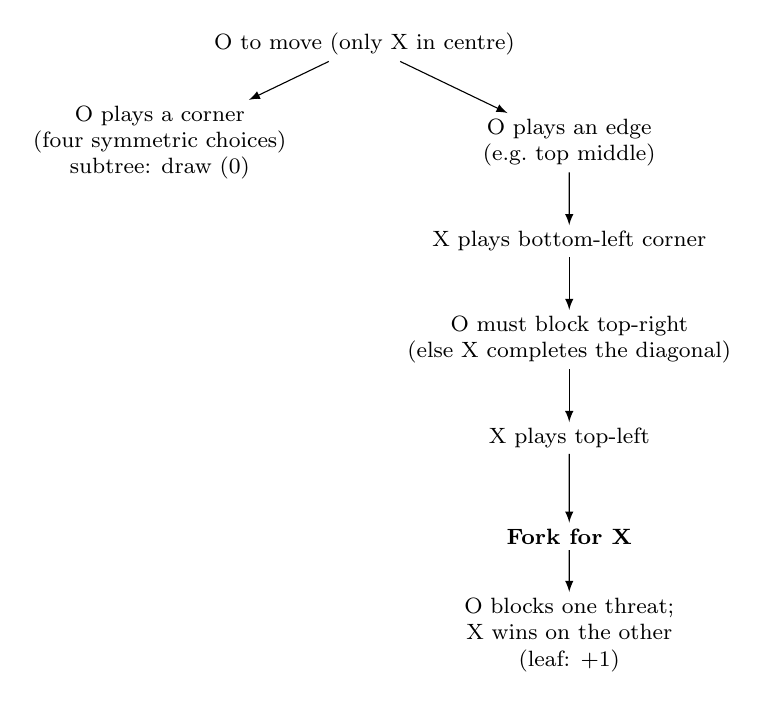
\begin{tikzpicture}[
  grow=down,
  level distance=1.25cm,
  every node/.style={align=center, font=\footnotesize, inner sep=2pt},
  edge from parent/.style={draw, -latex},
  level 1/.style={sibling distance=5.2cm},
  level 2/.style={sibling distance=5.2cm},
  level 3/.style={sibling distance=2.6cm},
  level 4/.style={sibling distance=2.6cm},
  level 5/.style={sibling distance=2.2cm}
]
\node {O to move (only X in centre)}
  child { node {O plays a corner\\(four symmetric choices)\\subtree: draw (\(0\))} }
  child { node {O plays an edge\\(e.g.\ top middle)}
    child { node {X plays bottom-left corner}
      child { node {O must block top-right\\(else X completes the diagonal)}
        child { node {X plays top-left}
          child { node {\textbf{Fork for X}}
            child { node {O blocks one threat;\\X wins on the other\\(leaf: \(+1\))}
            }
          }
        }
      }
    }
  };
\end{tikzpicture}
\end{center}

\noindent
After X's last move in that line, the board is
\begin{center}
\begin{tabular}{|c|c|c|}
\hline
X & O & O \\
\hline
\(\cdot\) & X & \(\cdot\) \\
\hline
X & \(\cdot\) & \(\cdot\) \\
\hline
\end{tabular}
\end{center}
\noindent
Now X simultaneously threatens two winning moves on the next turn: filling the
bottom middle square completes the bottom row, and filling the middle right square
completes the right column. O can answer at most one of those squares, so X
wins on the move after that. That position is a \emph{fork}: two lines each
missing one X, and O cannot block both.

At the root, O chooses a \emph{minimum} over the children's values; the edge
branch carries value \(+1\) for X, the corner branch \(0\). So O must take a
corner reply (on a diagonal through the centre), not an edge, or X wins.
